
\section{Ball and plate physical model}
\label{sec:sysmodel}

In order to present the mathematical model of the ball and plate system,
Figure~\ref{fig:model} shows the $xz$ view of the coordinate
system, introducing the needed parameters to define.

\begin{figure}[htb]
  \centering
  \psfrag{O}[bc]{\small$O$}
  \psfrag{A}[bc]{\small$A$}
  \psfrag{B}[bc]{\small$B$}
  \psfrag{rb}[bc]{\small$r_b$}
  \psfrag{q}[bc]{\small\ \ \ \ $\theta_x$, $\omega_x$, $\dot{\omega}_x$}
  \psfrag{ball}[bc]{\small$x, \dot{x}, \ddot{x}$}
  \psfrag{h}[bc]{\small$h$}
  \psfrag{N}[bc]{\small$\overline{N}$}
  \psfrag{F}[bc]{\small$\overline{F}$}
  \psfrag{mg}[bc]{\small$m\overline{g}$}
  \psfrag{x}[bc]{\small$\hat{x}$}
  \psfrag{z}[bc]{\small$\hat{z}$}
  \psfrag{plate}[bc]{\small$plate$}
  \psfrag{equi}[bc]{\small$equilibrium$}
  \psfrag{actuator}[bc]{\small$actuator$}
  \includegraphics[width=0.9\columnwidth]{physical_model.eps}
  \caption{$xz$ view of the ball and plate physical model.}
  \label{fig:model}
\end{figure}

\noindent The $yz$ view is identical to the $xz$
view, considering $\hat{y}$, $y$, $\dot{y}$, $\ddot{y}$, $\theta_y$,
$\omega_y$, $\dot{\omega}_y$ in place of $\hat{x}$, $x$, $\dot{x}$,
$\ddot{x}$, $\theta_x$, $\omega_x$ and $\dot{\omega}_x$, respectively.
Hence, the $yz$ view is omitted.

The fixed joint $O$, situated in the middle of the plate,
allows the surface to rotate around it within a specific angle range.
Moreover, the actuator and the plate are not joint directly as an arm
is inserted between them. The junction is length $h$, connecting the actuation
point $A$ and the actuated point $B$.

In order to simplify the computation, both the sliding and rolling frictions are
considered negligible.
%, so the ball equation takes into account only the rolling
%on the incline and the inertia due to the plate rotation.

The complete set of equations is continuos, non-linear and couples the two modes
of motion. After a discretization and linearization process about the operating
point, which is the equilibrium configuration
($x = y = \theta_x = \theta_y = 0$), the equations of motion for the ball,
along the $x$ and $z$ axis, are the following:

\begin{align*}
\ddot{x}[k] &= \frac{5}{7}\ g\ sin (\theta_x[k]) - \left ( r_b + \frac{5}{7}\ h \right ) \dot{\omega}_x[k]\\
%\frac{7}{5} \ddot{y} + \left ( \frac{7}{5} r_b + h \right ) \dot{\omega}_y &= g sin (\theta_y)
m\ddot{z}[k] &= N - mg\ cos(\theta_x[k]) = 0\\
%\dot{x}[k] &= \frac{ x[k] - x[k-1] } {\Delta t}\\
\dot{x}[k] &= \ddot{x}[k] \Delta t + \dot{x}[k-1]\\
x[k] &= \dot{x}[k] \Delta t + x[k-1]\\
\omega[k] &= \frac{ \theta[k] - \theta[k-1] } {\Delta t}\\
\dot{\omega}[k] &= \frac{ \omega[k] - \omega[k-1] } {\Delta t}
\end{align*}

Where $\Delta t$ is the control period (the time elapsed since the previous
control event until the actual). The first two equations are computed
according to the Newton's laws and the last four by the classical kinematic
formulas, assuming a motion uniformly accelerated during each $\Delta t$.

Note that linearizing decouples the two modes of motion.
Thus, the system can be treated as two different systems operating
simultaneously. Hence, similar but independent controllers can be used for
controlling each coordinate of the ball motion.
This lets us to design only one controller as the other one is exactly the same.
As the desired movements of the ball are only on the $xy$ plane,
the vertical acceleration (along $z$) is set equal to $0$.

% end section

